\section{Conception du Jeu BabylonJS}

Le troisième et dernier jeu de notre suite est incontestablement le projet le plus ambitieux et le plus complexe sur le plan technique de notre rendu. L'objectif était de concevoir un jeu de stratégie hybride en trois dimensions, fusionnant les mécaniques économiques et de placement d'un \textit{Auto-Chess} (inspiré de \textit{Teamfight Tactics}) avec les règles de déplacement du jeu d'échecs traditionnel. Pour soutenir une telle architecture, nous avons abandonné les configurations classiques au profit de \textit{Vite}, un outil de construction moderne et ultra-rapide. L'utilisation de Vite s'est avérée indispensable pour gérer efficacement le remplacement de modules à chaud (HMR) durant le développement, tout en offrant un empaquetage hautement optimisé pour nos ressources volumineuses, nos modèles tridimensionnels et nos modules compilés.

% ==========================================
% INSERTION DU DIAGRAMME 1 : CŒUR & VITE
% ==========================================
\FloatBarrier
\begin{figure}[H]
	\centering
	% Remplacez par le nom de votre fichier exporté
	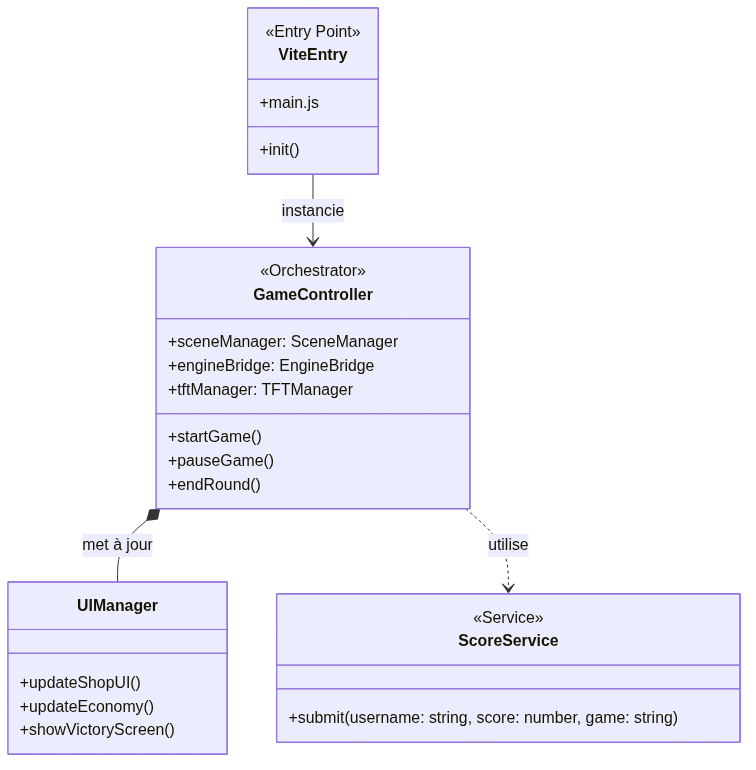
\includegraphics[width=0.8\textwidth]{babylon_1.png}
	\caption{Architecture principale et orchestration via l'environnement Vite}
	\label{fig:babylon_core}
\end{figure}
\FloatBarrier

La couche visuelle repose entièrement sur le framework BabylonJS, qui nous a permis de générer une scène tridimensionnelle performante exécutée directement dans le navigateur. La conception de cette couche est encapsulée dans un gestionnaire de scène dédié qui gère l'initialisation du moteur de rendu, le placement des caméras orbitales et le calcul de l'éclairage dynamique. Par-dessus cette scène, un chargeur de ressources asynchrone s'occupe de récupérer, de décoder et de mettre en cache nos modèles de pièces personnalisées au format GLB ou STL depuis le répertoire public. Les pièces sont ensuite liées à des objets logiques capables de transposer les coordonnées d'une grille d'échiquier mathématique abstraite vers des vecteurs spatiaux réels dans l'univers 3D, tout en gérant les animations de déplacement ou d'attaque.

% ==========================================
% INSERTION DU DIAGRAMME 2 : RENDU 3D
% ==========================================
\FloatBarrier
\begin{figure}[H]
	\centering
	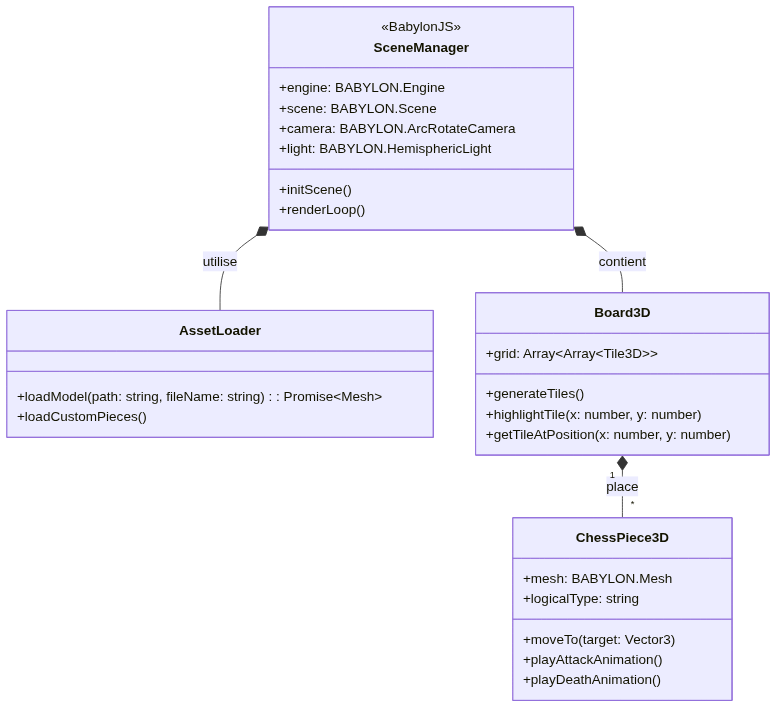
\includegraphics[width=0.8\textwidth]{babylon_2.png}
	\caption{Sous-système de rendu 3D et chargement asynchrone des modèles}
	\label{fig:babylon_3d}
\end{figure}
\FloatBarrier

La véritable complexité de ce projet réside toutefois dans son intelligence artificielle. Plutôt que de développer un algorithme d'échecs en JavaScript, ce qui aurait été bien trop lent, nous avons intégré \textit{Stockfish}, le moteur d'échecs open-source le plus puissant au monde. Pour ce faire, nous avons utilisé une version du moteur originellement écrit en C++, compilée en WebAssembly (WASM). Cette intégration a exigé la conception d'un pont de communication robuste. Le moteur WebAssembly s'exécute de manière isolée dans un \textit{Web Worker} afin de ne pas bloquer le fil d'exécution principal du navigateur gérant le rendu à soixante images par seconde. Le contrôleur du jeu traduit l'état actuel du plateau en notation Forsyth-Edwards (FEN), l'envoie au travailleur asynchrone, puis parse la réponse du moteur WASM pour animer les pièces adverses. Adapter ce moteur rigide à nos propres règles de pièces personnalisées et à notre plateau a constitué un défi architectural majeur.

% ==========================================
% INSERTION DU DIAGRAMME 3 : WEBASSEMBLY
% ==========================================
\FloatBarrier
\begin{figure}[H]
	\centering
	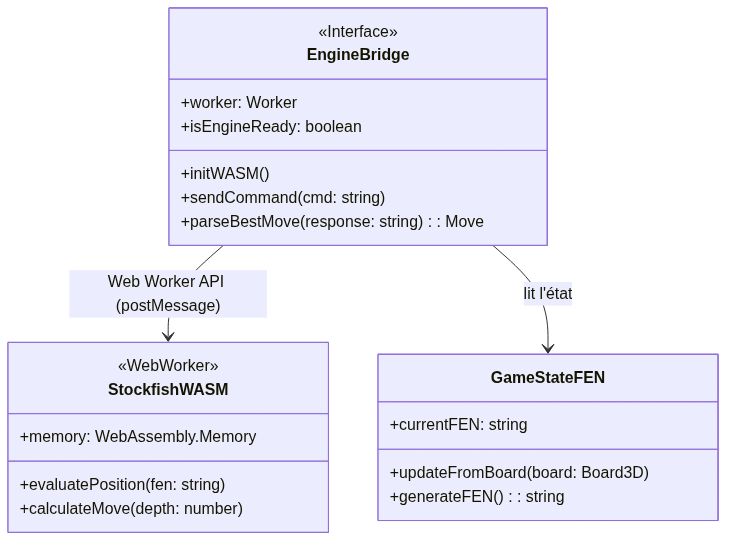
\includegraphics[width=0.8\textwidth]{babylon_3.png}
	\caption{Pont de communication asynchrone avec le moteur WebAssembly (Stockfish)}
	\label{fig:babylon_wasm}
\end{figure}
\FloatBarrier

Enfin, pour transformer ce simple jeu d'échecs en un véritable \textit{Auto-Chess}, nous avons implémenté une surcouche logique indépendante de la 3D et du moteur Stockfish. Cette couche est subdivisée en plusieurs gestionnaires spécialisés. Un gestionnaire d'économie calcule les revenus passifs, les intérêts et l'or généré par les séries de victoires ou de défaites. Un gestionnaire de boutique propose un choix aléatoire de pièces personnalisées à acheter entre chaque manche de combat. De plus, un gestionnaire de synergies analyse la composition de l'armée du joueur sur le plateau pour appliquer des modificateurs mathématiques globaux, affectant les calculs lors de la résolution du combat par WebAssembly. Cette stricte séparation des préoccupations permet au jeu de fonctionner par phases distinctes (draft et combat) sans créer de couplage fort entre l'interface utilisateur, la logique économique et les calculs du moteur.

% ==========================================
% INSERTION DU DIAGRAMME 4 : AUTO-CHESS LOGIC
% ==========================================
\FloatBarrier
\begin{figure}[H]
	\centering
	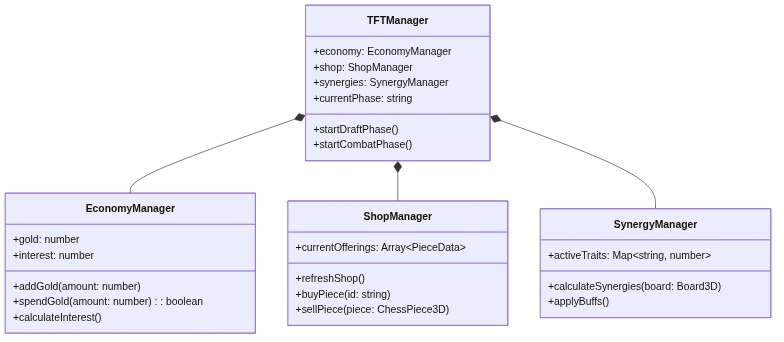
\includegraphics[width=0.8\textwidth]{babylon_4.png}
	\caption{Mécaniques Auto-Chess : Économie, Boutique et Synergies}
	\label{fig:babylon_tft}
\end{figure}
\FloatBarrier